%
% File eacl2017.tex
%
%% Based on the style files for ACL-2016
%% Based on the style files for ACL-2015, with some improvements
%%  taken from the NAACL-2016 style
%% Based on the style files for ACL-2014, which were, in turn,
%% Based on the style files for ACL-2013, which were, in turn,
%% Based on the style files for ACL-2012, which were, in turn,
%% based on the style files for ACL-2011, which were, in turn, 
%% based on the style files for ACL-2010, which were, in turn, 
%% based on the style files for ACL-IJCNLP-2009, which were, in turn,
%% based on the style files for EACL-2009 and IJCNLP-2008...

%% Based on the style files for EACL 2006 by 
%%e.agirre@ehu.es or Sergi.Balari@uab.es
%% and that of ACL 08 by Joakim Nivre and Noah Smith

\documentclass[11pt]{article}
\usepackage{eacl2017}
\usepackage{times}
\usepackage{url}
\usepackage{latexsym}
\usepackage{natbib}
\usepackage{amsmath}
\usepackage{subfigure}
\usepackage{graphicx}

\hyphenation{CCCRE}

% \eaclfinalcopy % Uncomment this line for the final submission
%\def\eaclpaperid{***} %  Enter the acl Paper ID here

%\setlength\titlebox{5cm}
% You can expand the titlebox if you need extra space
% to show all the authors. Please do not make the titlebox
% smaller than 5cm (the original size); we will check this
% in the camera-ready version and ask you to change it back.

\newcommand\BibTeX{B{\sc ib}\TeX}

\title{Learning to Negate Adjectives with Bilinear Models}
% Learning to Negate Adjectives with Relational Antonym Encoders
% Learning to Negate Adjectives with Continuous Class-Conditional Relational Encoders

\author{First Author \\
  Affiliation / Address line 1 \\
  Affiliation / Address line 2 \\
  Affiliation / Address line 3 \\
  {\tt email@domain} \\\And
  Second Author \\
  Affiliation / Address line 1 \\
  Affiliation / Address line 2 \\
  Affiliation / Address line 3 \\
  {\tt email@domain} \\}

\date{}

\begin{document}
\maketitle
\begin{abstract}
We learn a mapping that negates adjectives by
predicting an adjective's antonym in an arbitrary word embedding
model. We show that both linear models and neural networks improve on
this task when they have access to a vector representing the semantic
domain of the input word, e.g. a centroid of temperature words when
predicting the antonym of `cold'. We introduce a continuous
class-conditional bilinear neural network which is able to negate
adjectives with high precision.
\end{abstract}

\section{Introduction}

Identifying antonym pairs such as {\it hot} and {\it cold} in a vector space model is a challenging task.
Previous work has explored learning or retrofitting specialised embeddings that push antonyms further apart than synonyms
% in the vector space 
\citep{pham:15,nguyen:16,mrksic:16}, or using
unsupervised measures to distinguish antonym pairs from other
binary lexical relations \citep{santus:15}. 
% However, none of these
% methods provide us with a negation function which helps us locate an
% acceptable antonym for a given word in the space. 
However, these approaches do not offer a negation mapping which predicts an antonym for a given word, in an arbitrary word embedding model. 
%, given an arbitrary set of word embeddings.  This
% task is important for composing larger units of meaning, where a
% phrase such as {\it not cold} might need to be assigned a vector space
% representation.

In this paper we learn such a mapping.
% , an important subtask for composing larger units of meaning, where a phrase such as {\it not cold} might need to be assigned a vector space representation. 
We focus on negating adjectives, and treat negation as prediction of a
one-best antonym. For example, given the expression {\it not
  talkative} and the vector $\overrightarrow{\textit{talkative}}$, the mapping should return a word from the set {\it quiet, taciturn,
  uncommunicative}, etc.
% More nuanced treatmeants of antonym negation are possible; e.g. the meaning of {\it not
%   hot} can include {\it cool,
%   tepid, warm} etc. depending on the context \citep{hermann:13}.
% [TODO  Baroni] [TODO maybe a linguistic cite]
% Previous work on antonymy has suggested that, while antonyms are
% distributionally similar, there are differences which can be
% exploited. 
Antonym pairs share a domain---e.g. {\it   temperature}, but differ in their value---e.g. {\it coldness}
\citep{turney:12,hermann:13}. Negation must alter the value while retaining the domain.

In this paper we exploit the semantic neighbourhood of an adjective
as a stand-in for the domain. We hypothesize that the relevant
features for negating, say, a temperature adjective, differ from those
for an emotion adjective. Therefore, our negation mappings make use of a
vector at the centroid of words related to the input.
% representing the semantic domain of the input word. 
% Moreover, a negation function must be (informally) involuntory,
% i.e. its own inverse, so it must detect the ``direction'' in which the
% input word is more extreme than the neutral vector. 
This approach is inspired by \citet{kruszewski:16},
 who find that nearest neighbours in a vector space are a good approximation for human judgements of possible alternatives to negated nouns.

We also introduce a variant of a bilinear relational neural network architecture which has proven successful in 
identifying image transformations in computer vision. Our model outperforms several baselines on a
multiple choice antonym selection task, and learns to produce a
one-best antonym with high precision.


\section{Relational Encoders}

\begin{figure*}[h!t]
\centering
\subfigure[Relational Autoencoder]{
 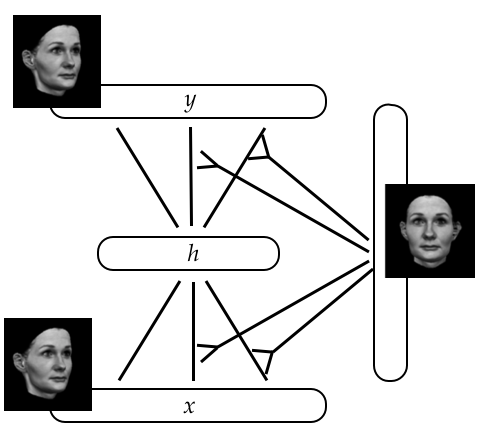
\includegraphics[width=0.25\textwidth]{rae}
}
\quad
\subfigure[CCRAE]{
 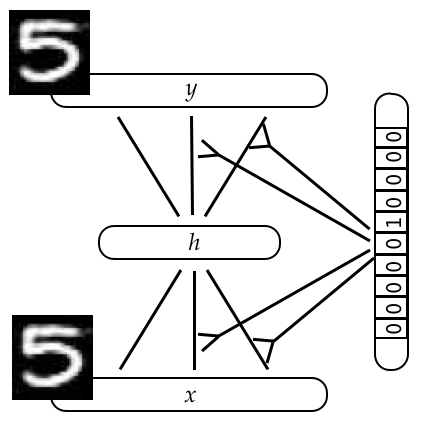
\includegraphics[width=0.22\textwidth]{ccae}
}
\quad
\subfigure[CCCRE]{
 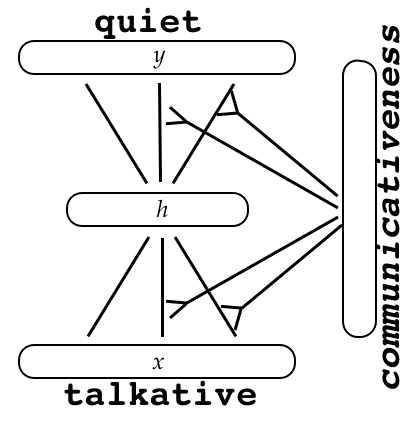
\includegraphics[width=0.21\textwidth]{cccre}
}
\label{f:arch}
\vspace{-4mm}
\caption{Neural network architectures and training signal for (a) RAE \citep{memisevic:13}, (b) Class-Conditional RAE \citet{rudy:15}, and Continuous Class-Conditional RAE (this paper). Figures based on \citet{memisevic:13}.}
\end{figure*}


\subsection{Relational Autoencoders: Background}

Relational autoencoders (RAE), also known as gated autoencoders (GAE),
have been used in computer vision to learn representations of
transformations between images, such as rotation or translation \citep{memisevic:07,memisevic:12,memisevic:13}. RAEs
are a type of {\it gated network}, which contains multiplicative connections
between two related inputs.
%  are used for prediction or representation learning. 
The ``gating'' of one image vector by another allows feature detectors to concentrate on the correspondences between the related images, rather than being distracted by the differences between untransformed images. See Figure~\ref{f:arch}(a). 
Multiplicative connections involve
% The key is the use of bilinear connections; 
a weight for every pair of units in the input vector and gate vector. For an overview of RAEs see \citet{memisevic:13,sigaud:15}.
% The connections are known as bilinear because for an image x and its rotated image y, f(y) is a linear function of x, and vice versa.
% The connections are symmetric, but one input is usually considered primary and the other the gate.

RAE gates perform a somewhat different function than LSTM gates \citep{lstm}. Both architectures use a nonlinearity to modulate the contents of a product; in an RAE this is an outer (bilinear) product while in an LSTM it is a Hadamard (element-wise) product. However, LSTM memory gates represent an internal hidden state of the network, while RAE gates are part of the network input.

An Autoencoder (AE) can be defined as in Eq~\ref{eq:AE} (we omit bias terms for simplicity), where $\mathrm{W_e}$ are the encoder weights and $\mathrm{W_d}$ are the decoder weights. In autoencoders, weights are typically tied so that $\mathrm{W_d} = \mathrm{W_e}^T$.

\vspace{-7mm}
\begin{equation}
\begin{split}
h & = f(x) = \sigma (\mathrm{W_e}x ) \\
y & = g(h) = \mathrm{W_d}h
\end{split}
\label{eq:AE}
\end{equation}
\vspace{-5mm}

\noindent For an RAE, we have two inputs $x$ and $z$. Instead of a weight matrix $W$ we have a weight tensor $\overline{\mathrm{W}} \in R^{n_H \times n_X \times n_Z}$.  The RAE is defined in Eq~\ref{eq:RAE}.

\vspace{-7mm}
\begin{equation}
\begin{split}
h & = f(x, z) = \sigma ((\overline{\mathrm{W_e}}z)x) \\
y & = g(h, z) = \sigma ((\overline{\mathrm{W_d}}h)z)
\end{split}
\label{eq:RAE}
\end{equation}
\vspace{-5mm}

\citet{rudy:15} introduce a class-conditional gated autoencoder in which the gate is a one-hot class label, rather than a transformed version of the input image. For example, in the MNIST task the label represents the digit. Effectively, an autoencoder is trained per class, but with weight sharing across classes. See Figure~\ref{f:arch}(b).

\subsection{Continuous Class-Conditional Relational Encoders}

Our bilinear model is a continuous class-conditional relational encoder (CCCRE). The model architecture is the same as an RAE with untied encoder and decoder weights. However, the training signal differs from a classic RAE in two ways. First, it is not an autoencoder, but simply an encoder, because it is not trained to reproduce the input but rather to transform the input to its antonym. Second, the encoder is class-conditional in the sense of \cite{rudy:15}, since the gate represents the class.
% . In a classic RAE the input and gate are related according to a transformation, but in a class-conditional AE the gate represents the class. 
Unlike the one-hot gates of \cite{rudy:15}, our gates are real-valued, representing the semantic domain of the input vector. See Figure~\ref{f:arch}(c). The intuition behind our model is that it learns to negate a word in the context of that word's semantic domain.

\section{Experiments}

\subsection{Models}

We compare the CCCRE with several baselines. The simplest is cosine similarity in the original vector space. We train a linear model ({\bf Linear}) which maps the input word to its antonym, an Untied Encoder ({\bf UE}) with a bottleneck hidden layer, and a shallow feed-forward model ({\bf FF}) with a wide hidden layer rather than a bottleneck. To test whether the semantic domain is helpful in learning negation, each of these models has a {\bf Concat} version in which the input consists of the concatenated input word and gate vectors. 
% {\bf UE-Concat} has 300 hidden units and {\bf FF-Concat} has 600. We did not find using dropout to improve performance in any of our models.

\subsection{Experimental Settings}

We use publicly-available\footnote{\url{https://code.google.com/archive/p/word2vec/}} 300-dimensional embeddings trained on part of the Google News dataset using skip-gram with negative sampling (SGNS) \citep{mikolov:13}.
Antonym training data was obtained from WordNet \citep{wordnet} (hereafter WN), resulting in approximately 20K training pairs.
% We used the antonym relation for WN adjectives, and expanded the initial list of antonym pairs with WN synonyms of each word in the pair. This resulted in approximately 20K (input word, target word) training pairs. 
We exclude any antonym pair with the input word in the test set.

Gate vectors were obtained under three conditions. In the {\bf
  standard} condition we use all WN cohyponyms of an input word. If
there are fewer than ten, we make up the difference with nearest neighbours
from the 
% original
vector space. The gate vector is 
% calculated as 
the vector centroid of the resulting word list.

% We did not exclude cohyponyms of the test input words, since the theory is that the network needs these examples to learn the gates / contexts. That is, if 'cold' is in the test set, the model learns how to negate it by learning how to negate other temperature words.

% Neutral context gates were obtained under three conditions. In the {\bf standard} condition we take all WordNet cohyponyms of the adjective
% sense of input word $w$, where cohyponyms include: other lemmas in the synset, children of attribute, synonyms, antonyms, synonyms of the antonyms, similar-tos. If there were fewer than 10 cohyponyms in WordNet, we increased the number to 10 with non-overlapping nearest neighbours from the original vector space. The gate is the centroid of these vectors.

In the {\bf unsupervised} gate condition we do not use WN, but rather the ten nearest neighbours from the 
% original 
vector space. 
% However, the target antonym is still supervised. 
In the {\bf restricted} condition, we remove all WN cohyponyms of test input words from the training data, e.g. {\it hot, cool, tepid} etc. if {\it cold} is a test word.
% This is to test how important it is to have training examples with similar gates. 
% For example, if {\it cold} is a test word, we remove {\it hot, cold, tepid, cool} etc. from the training data.

% Hyperparameters including hidden layer size, minibatch size and number of epochs were tuned on the GRE development set. All models were optimized using AdaDelta to minimize Mean Squared Error loss. 
Hyperparameters were tuned on the GRE development set (Sec~\ref{sec:eval}). All models were optimized using AdaDelta ($\rho = 0.95$) to minimize Mean Squared Error loss. The FF and CCCRE networks have hidden layers of 600 units, while UE has 150 and UE-Concat has 300. Minibatch size was 48 for CCCRE and 16 for all other networks. The linear models were trained for 100 epochs, FF networks for 400, UE for 300, and CCCRE for 200.

\subsection{Evaluation}
\label{sec:eval}

% We evalute our models with two experiments. 
Experiment 1 uses the Graduate Record Examination (GRE) questions of \citet{mohammad:13}. The task, given an input word, is to pick the best antonym from five options. An example 
% from the development set 
is shown in (\ref{eqn:gre-ex}), where the input word is {\it piquant} and the correct answer is {\it bland}. We use only those questions 
% restrict the questions to those 
where both input and target are adjectives.

\vspace{-6mm}
\begin{equation}
\begin{split}
\textrm{piquant:\ \ } & \textrm{(a) shocking (b) jovial (c) rigorous} \\[-1mm]
& \textrm{(d) merry (e) {\bf bland}}
\label{eqn:gre-ex}
\end{split}
\end{equation}
\vspace{-6mm}

We evaluate a model by predicting an antonym vector for the input word, and choosing the multiple choice option with the smallest cosine distance to the predicted vector. We report accuracy, i.e. percentage of questions answered correctly.

Experiment 2 evaluates the precision of the models. 
A natural criterion for the success of a negation mapping is whether the model returns a good antonym at rank 1, or several good antonyms at rank 5, rather than returning any particular antonym as required by the GRE task.

% Recall that our goal is to negate an adjective given its word vector. A natural criterion for success is 

We use two datasets: the GRE test set ({\bf GRE}), and a set of 99 adjectives and their
antonyms from a crowdsourced dataset collected by Lenci and Benotto
acccording to the guidelines of \citet{walde:13} ({\bf LB}). For each input word we retrieve the five nearest neighbours of the model prediction and 
% check against a gold standard whether each neighbour is an acceptable antonym.
check them against a gold standard.
Gold standard antonyms for a word include its antonyms from the test sets and WN. Following \citet{gorman:05}, to minimise false negatives we improve the coverage of the gold standard by expanding it with antonyms from 
% the online version of 
Roget's 21st Century Thesaurus, Third
Edition.\footnote{\url{http://thesaurus.com}} We report precision at
ranks 1 and 5.


\section{Results and Discussion}
\begin{table}[t!]
\centering
\small
\begin{tabular}{lccc}
 & \multicolumn{3}{c}{\bf Training Condition} \\
\bf Method & \bf Stand. & \bf Unsup. & \bf Restr. \\
\hline
\hline
Random & 0.20 & --- & --- \\
Cosine & 0.50 & --- & --- \\
\hline
Linear & 0.56 & 0.56 & 0.53 \\
Linear-Concat & 0.66 & 0.59 & 0.63 \\
\hline
UE & 0.57 & 0.55 & 0.52 \\
UE-Concat & 0.63 & 0.58 & 0.61 \\
FF & 0.58 & 0.54 & 0.51 \\
FF-Concat & 0.65 & 0.56 & 0.63 \\
\hline
CCCRE & \bf 0.69 & \bf 0.60 & \bf 0.65 \\
\end{tabular} 
\caption{Accuracy on the 367 multiple-choice adjective questions in the GRE test set.}
\label{t:gre}
\end{table}

\begin{table*}[t!]
\centering
\small
% \setlength\tabcolsep{1.5pt}
\begin{tabular}{lcc|cc|cc||cc|cc|cc}
& \multicolumn{6}{c||}{\bf GRE} & \multicolumn{6}{c}{\bf LB} \\
& \multicolumn{2}{c|}{\bf Stand.} & \multicolumn{2}{c|}{\bf Unsup.} & \multicolumn{2}{c||}{\bf Restr.} & \multicolumn{2}{c|}{\bf Stand.} & \multicolumn{2}{c|}{\bf Unsup.} & \multicolumn{2}{c}{\bf Restr.} \\
\bf Method & \bf P@1 & \bf P@5  & \bf P@1 & \bf P@5  & \bf P@1 & \bf P@5  & \bf P@1 & \bf P@5  & \bf P@1 & \bf P@5  & \bf P@1 & \bf P@5  \\
\hline
\hline
Cosine & 0.05 & 0.07 & --- & --- & --- & --- & 0.13 & 0.10 & --- & --- & --- & --- \\
\hline
Linear & 0.36 & 0.29 & 0.34 & 0.29 & 0.32 & 0.28 & 0.29 & 0.25 & 0.30 & 0.24 & 0.29 & 0.23 \\
Linear-Concat & 0.39 & 0.33 & 0.43 & 0.34 & 0.36 & 0.31 & 0.33 & 0.28 & 0.31 & 0.27 & 0.32 & 0.27 \\
\hline
UE & 0.38 & 0.33 & 0.36 & 0.32 & 0.37 & 0.31 & 0.28  & 0.22 & 0.27 & 0.23 & 0.23 & 0.20 \\
UE-Concat & 0.38 & 0.33 & 0.43 & 0.38 & 0.27 & 0.31 & 0.33 & 0.28 & 0.34 & 0.27 & 0.28 & 0.25 \\
FF & 0.37 & 0.32 & 0.34 & 0.30 & 0.08 & 0.15 & 0.30 & 0.24 & 0.27 & 0.23 & 0.22 & 0.19 \\
FF-Concat & 0.36 & 0.30 & 0.46 & 0.40 & 0.37 & 0.34 & 0.34 &  0.26 & 0.28 & 0.26 & \bf 0.34 & 0.27 \\
\hline
CCCRE  & \bf 0.66 & \bf 0.49 & \bf 0.52 & \bf 0.42 & \bf 0.52 & \bf 0.38 & \bf 0.39 & \bf 0.32 & \bf 0.46 & \bf 0.32 & \bf 0.34 & \bf 0.30 \\
\end{tabular} 
\caption{Precision at ranks 1 and 5 on the GRE and Lenci and Benotto datasets.}
\label{t:prec}
\end{table*}

\begin{table*}
\small
\centering
\begin{tabular}{lll}
\bf Method & \multicolumn{2}{l}{\bf Top 5 Predictions} \\
\hline
\hline
CCCRE & ornate: & {\bf unadorned, inelegant, banal}, oversweet, {\bf unembellished} \\
%      & anemic: & {\bf strong, solid, robust, buoyant, good} \\
      & ruthless: & {\bf merciful, compassionate, gentle, righteous, meek} \\
\hline
FF-Concat & ornate: & {\bf unadorned, unornamented}, overdecorated, {\bf elegant}, sumptuousness \\
%          & anemic: & {\bf strong}, lackluster, {\bf solid, robust}, tepid \\
          & ruthless:&  merciless, heartless, {\bf meek, merciful}, unfeeling \\
\end{tabular}
\caption{Samples of top five nearest neighbours of predicted antonym vectors for CCCRE and FF-Concat.}
\label{t:top5}
\end{table*}


Table~\ref{t:gre} shows the results of Experiment 1. A random baseline results in 0.20 accuracy. The cosine similarity baseline is already fairly strong at 0.50, suggesting that in general about two out of the five options are closely related to the input word.

Information about the semantic domain clearly provides useful information for this task, because the {\bf Concat} versions of the Linear, UE, and FF models achieve several points higher than the models using only the input word. The linear model achieves a surprisingly high 0.66 accuracy under standard training conditions.

CCCRE achieves the highest accuracy across all training conditions, and is the only model that beats the linear baseline, suggesting that bilinear connections are useful for antonym prediction.

All the models show a notable loss of accuracy in the {\bf unsupervised} condition,
% , where the gates are built from nearest neighbor vectors rather than WN cohyponyms, 
suggesting that 
% despite the findings of \citet{kruszewski:16}, 
the alternatives found in the vector neighbourhood are less useful than supervised gates.
% It is possible that their centroid is too close to the input vector to make a useful gate. 
Even in this setting, however, CCCRE achieves a respectable 0.60.
In the {\bf restricted} condition, 
% where cohyponyms of the test words are excluded from training, 
all non-Concat models perform near the cosine baseline, suggesting that in the standard setting they were memorising antonyms of semantically similar words. The Concat models and CCCRE retain a higher level of accuracy, indicating that they can generalise across different semantic classes.

Although CCCRE achieves the highest accuracy in Experiment 1, the GRE task does not really reflect our primary goal, namely to negate adjectives by generating a one-best antonym. CCCRE sometimes fails to choose the target GRE antonym, but still makes a good overall prediction. For input word {\it doleful}, the model fails to choose the GRE target word {\it merry}, preferring instead {\it sociable}. However, the top three nearest neighbours for the predicted antonym of {\it doleful} are {\it joyful, joyous}, and {\it happy}, all very acceptable antonyms. 
% Experiment 2 measures precision directly.
% This phenomenon is addressed in Experiment 2.

Table~\ref{t:prec} shows the results of Experiment 2. On the GRE dataset, under standard training conditions, CCCRE achieves an impressive P@1 of 0.66, i.e. two thirds of the time it is able to produce an antonym of the input word as the nearest neighbour of the prediction. All of the other models score less than 0.40. In the {\bf unsupervised} and {\bf restricted} training conditions CCCRE 
% retains the ability to give 
still predicts a one-best antonym about half the time.
% , much higher than the other models.
%, whereas few of the other models approach this level.

The LB dataset is more challenging, because it contains a number of words which lack obvious antonyms, e.g. {\it taxonomic, quarterly, morphological}, and {\it fiscal}. However, CCCRE still achieves the highest precision on this dataset. Interestingly, precision does not suffer as much in the less supervised trianing conditions, and P@1 even improves with the {\bf unsupervised} nearest neighbour gates. We speculate that nearest distributional neighbours correspond better than the WN ontology to the crowdsourced antonyms in this dataset.

Table~\ref{t:top5} shows sample predictions for the CCCRE and FF-Concat models. It can be seen that CCCRE has more antonyms at the highest ranks.


% [TODO: try to fit an example of the top 5 for CCCRE and one other model for an example word or two!]

% [TODO: we expect the network will have the hardest time negating adjs that don't have a good gate, i.e. a well-defined semantic neighbourhood. Look for some examples.]

\section{Related Work}

% \citet{widdows:03} introduces a binary negation function for vector
% spaces, e.g. {\it suit NOT lawsuit}, which is used for word sense
% disambiguation in Information Retrieval. 
% \citet{turney:12} and \citet{hermann:13}
% propose a multi-region vector representation that separates domain and
% value.
% but this does not allow negation of a word in an arbitrary
% vector space. 
\citet{pham:15,nguyen:16,mrksic:16} use WN and other ontologies to retrofit embeddings, or learn
embeddings with a secondary objective of pushing antonyms further apart than synonyms.
% , pushing synonyms closer
% together and antonyms further apart. 
% This improves the overall vector
% space and makes it more likely that close words will be synonyms, but
% does not provide a way to find antonyms in the
% space. 
\citet{santus:14a,santus:14b,santus:15} perform unsupervised synonym-antonym
discrimination using the relative salience of shared features. 
% This type of relation classification does
% not make it possible to negate an arbitrary word. 
\citet{mohammad:13} use a supervised
thesaurus-based method 
% augmented with co-occurrence statistics 
on the GRE task.
% (including nouns and verbs). 
% [TODO Maybe de Marneffe on adjective scales.]
\citet{pham:15} learn negation as a linear map, and find that it is more effective at predicting a one-best antonym when vectors have been specially trained for lexical contrast.
% on standard SGNS vectors and vectors trained with a lexical contrast objective, finding the map more effective at predicting a one-best antonym on the specialy trained vectors.

RAEs and related architectures have been used in computer vision for a number of applications including recognising transformed images \citep{memisevic:07}, 
recognising actions \citep{taylor:10}, 
learning invariant features from images and videos \citep{grimes:05,zou:12},
% , recognising human poses \cite{taylor:09}, 
and reconstructing MNIST digits and facial images \citep{rudy:15}.
\citet{wang:15} use RAEs for tag recommendation, but RAEs have not been widely used in NLP.


%  Turney (2008) proposed a supervised algorithm for the identification of several semantic relations, including synonyms and opposites. The algorithm relied on a training set of word pairs with class labels to assign the labels also to a testing set of word pairs. All word pairs were represented as vectors encoding the fruencies of co-occurrence in textual patterns extracted from a large corpus of web pages. He used the seuential minimal optimization (SMO) support vector machine (M) with a radial basis function (RBF) kernel (Platt, 1998) implemented in Weka (Waikato Environment for Knowledge Analysis) (Witten and Frank, 1999). In the discrimination between synonyms and opposites, the system achieved an accuracy of 75% against a majority class baseline of 65.4%. Mohammad et al. (2008) proposed a method for determining the degree of semantic contrast (i.e. how much two contrasting words are semantically close)  based on the use of thesauri categories and corpus statistics. For each target word pair, they used the co-occurrence and the distributional hypothesis to establish the degree of opposition. Their algorithm achieved an F-score of 0.7, against a random  baseline of 0.2. Mohammad et al. (2013) used an analogical method based on a given set of contrasting words to identify and classify different kinds of opposites by hypothesizing that for every opposing pair of words, A and B, there is at least another opposing pair, C and D, such that A is similar to C and B is similar to D. For example, for the pair
% . Given the existence of contrast, they calculated its degree relying on the
% co-occurrence
%  hypothesis. Their approach outperformed other state-of-the-art measures



\section{Conclusion}

We have shown that a representation of the semantic domain improves antonym prediction in linear and non-linear models, and that the multiplicative connections in a bilinear model are effective at learning to negate adjectives with high precision. 
% In the broader context of modelling closed-class function words, it is perhaps not too farfetched to imagine that a specialised network with multiplicative connections might be necessary to model these kinds of words.

Our implementation uses a full tensor for the bilinear layer, and takes several hours to train on a GPU. Future work will exploit options for reducing the number of parameters to be learned \citep{alain:13} and address negation of nouns and verbs,
where negation is more likely to involve a set of alternatives than a one-best antonym.
% where negation is more likely to involve a probability distribution over alternatives---e.g. {\it didn't run} might mean {\it walk} or {\it amble}---rather than predicting a single best antonym.

\clearpage

\bibliographystyle{myplainnat}
\bibliography{eacl2017}
% \bibliographystyle{eacl2017}


\end{document}
